\section{\texttt{RankSwappingFilter}}
\label{Implementation:RankSwapping}

The rank swapping SDC method described in~\sref{Theory:SDCMethods:RankSwapping} is implemented by the \texttt{RankSwappingFilter} class. We must notice that it is a very naïve implementation and certainly not the fastest of the filters. As we will discuss later, future work is needed to enhance the performance of this filter.

\subsection{Design}
\label{Implementation:RankSwapping:Design}

The \texttt{RankSwappingFilter} is the second \textit{buffered filter} that has been implemented in this project (see~\sref{Implementation:BufferedFilter}). Almost the same data structures (the $W$, $W'$ and $A$ buffers) used by the \texttt{MicroAggregationFilter} are used by the rank swapping algorithm. The main difference with respect to the microaggregation algorithm is that the set $A$, used to know whether or not an \textit{instance} has already been anonymized, is now used to know whether or not a \textit{value} $w_{ij}'$ (this is, the $j$-th attribute value of the $i$-th instance in $W'$) has been \textit{swapped} or not. Summarizing, we say that $w_{ij}'$ has been swapped if $w_{ij}' \in A$.

\begin{figure}
\centering
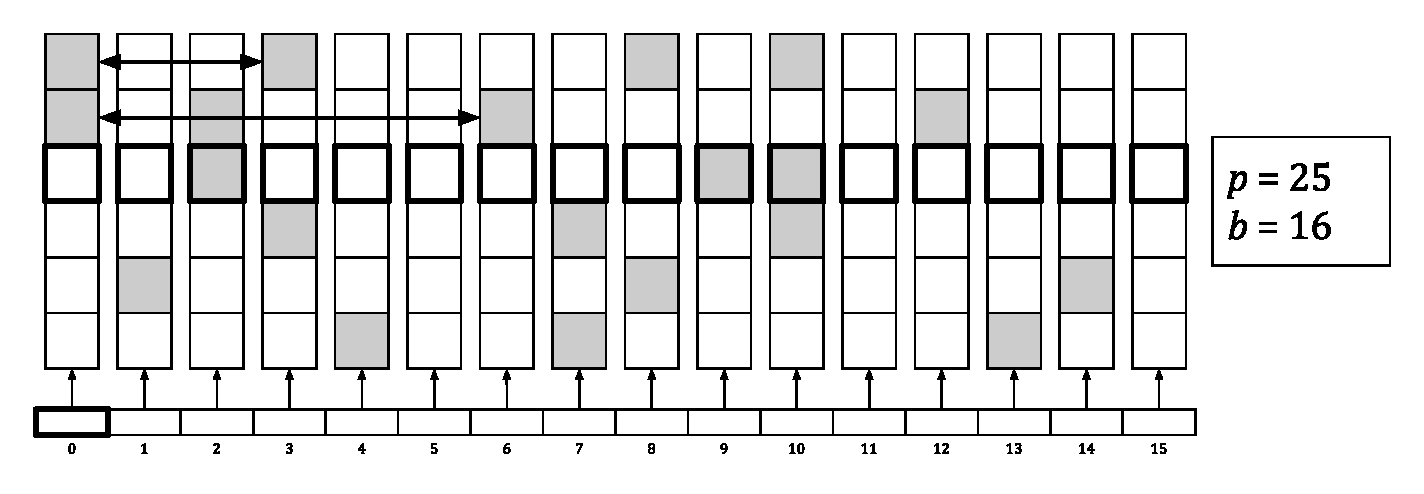
\includegraphics[width=1.0\linewidth]{figures/rank-swapping-schematic-1.pdf}
\caption[Rank swapping algorithm schematic.]{Rank swapping algorithm schematic. Two attributes of the target record (position 0) have already been \textit{rank swapped} with other values from instances in the buffer. The variable being now processed is highlighted.}
\end{figure}

\begin{figure}
\centering
\makebox[\textwidth][c]{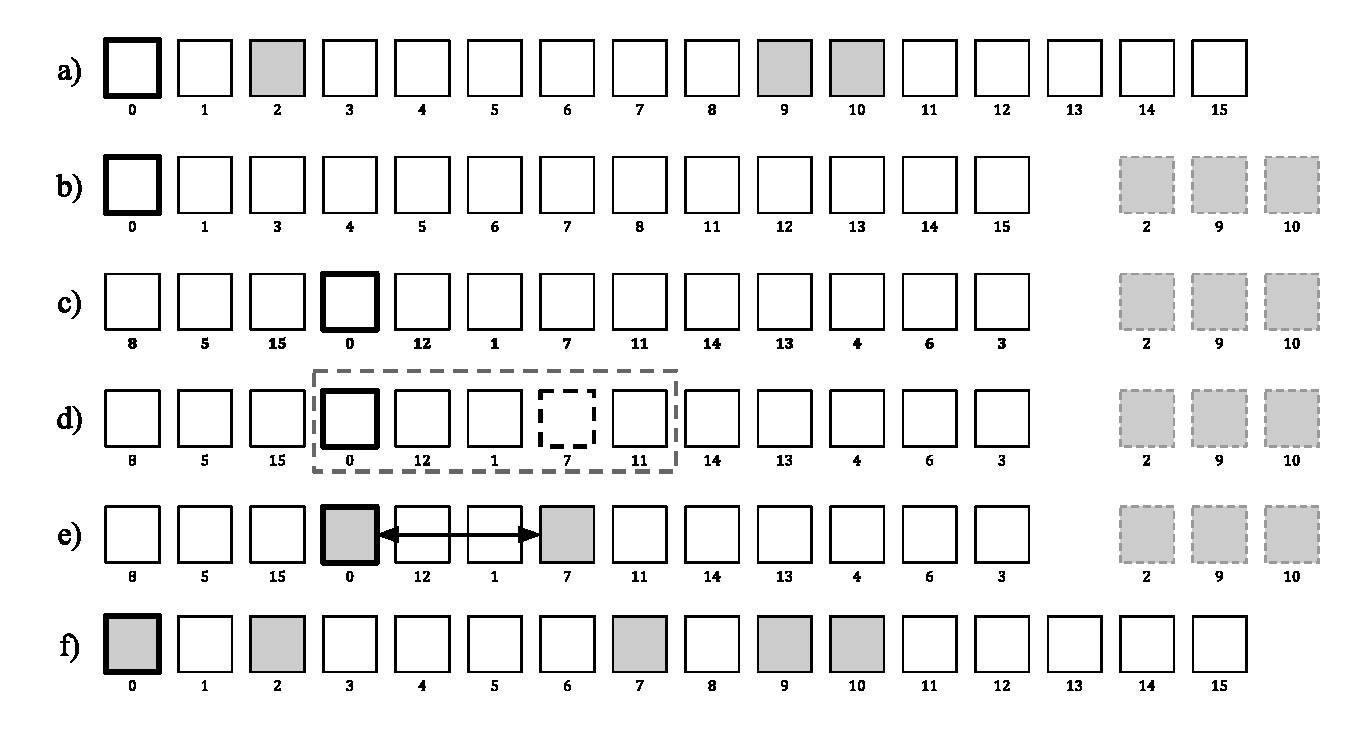
\includegraphics[width=1.1\linewidth]{figures/rank-swapping-schematic-2.pdf}}
\caption[Rank swap of an attribute.]{Rank swap of a single attribute for a target instance $\tau$. First, the non already swapped values of the attribute are filtered from the instances in the buffer $W$ (b) and are ranked, i.e., sorted (c). A maximum swap range is calculated using the $p$ parameter (d) and a value within this range is selected to perform the swap (e). Finally, the vector of values is returned in the original order they were in the buffer (f).}
\label{fig:rank-swapping-schematic-2}
\end{figure}

The design of this SDC method follows almost exactly the explanation given in the theoretical background chapter (\sref{Theory:SDCMethods:RankSwapping}): for each instance processed from the stream, values of each variable $j$ are ranked in ascending order, this is, they are \textit{sorted}. Each ranked value is then swapped with another ranked value, randomly chosen within a restricted range, controlled by the input parameter $p$, which denotes that swapped values cannot differ more than $p\%$ of the total number of records. A more formal description of its implementation is given in~\alref{al:rank-swapping}, along with its auxiliar procedure \texttt{selectSwap()} (see~\procref{al:select-swap}). Also, a more visual explanation is shown in~\fref{fig:rank-swapping-schematic-2}.

\begin{algorithm}[H]
\KwData{$W', A, p$}
\KwResult{the target instance $\tau$ is anonymized}
\Begin{
	$\tau \leftarrow w_0'$\;
	\For{$j \in \mathrm{attributes}(\tau)$}{
		$\gamma \leftarrow \mathrm{selectSwap}(W',p,j)$\;
		$\sigma \leftarrow w_\gamma'$\;
		$\mathrm{swap}(\tau_j, \sigma_j)$\;
		$A \leftarrow A \cup \tau_j \cup \sigma_j$\;
	}
}
\caption{Rank Swapping\label{al:rank-swapping}}
\end{algorithm}

\begin{procedure}
\KwData{$W'$ buffer, $p$ parameter and $j$ attribute}
\KwResult{the index $\gamma$ of the instance with which the swap will be done}
\Begin{
	$V \leftarrow \mathrm{Vector}(\{\langle w_{ij}', i \rangle~\vert~0 \leq i \leq b-1,~w_{ij}' \notin A\})$\;
	\tcp{Notice that, by construction, $\langle \tau_j, 0\rangle \in V$}
	$V^* \leftarrow \mathrm{sort}(V)$ \tcp{sort by \textit{value}, not by index}
	$t \leftarrow V^*.index(\langle \tau_j, 0\rangle)$\;
	$r \leftarrow 1 + \mathrm{Random}.uniform()~\mathrm{mod}~(p \cdot b~/~100)$ \tcp{$r \in [1, p\% \cdot b] $}
	$s \leftarrow 0$\;
	\eIf{$t + r < V^*.size() $}{
		$s \leftarrow t + r$\;
	}{
		$s \leftarrow V^*.size() - 1$\;
	}
	\tcp{$s$ is the index of the selected value-index pair to be swapped}
	$\langle \cdot,\gamma \rangle \leftarrow V^*[s]$\;
	\KwRet{$\gamma$}\;
}
\caption{selectSwap($W',p,j$)\label{al:select-swap}}
\end{procedure}

If we examine the previous rank swapping algorithm in detail, we can estimate its computational complexity. The cost of swapping a value of an attribute is, basically, that of sorting all of its values: $O(b \cdot \mathrm{log}(b))$, where $b$ is the size of the buffers $W$ and $W'$. Each of the $n$ instances of the stream will have its $m$ attributes rank swapped with those of another record; therefore, the total complexity of the algorithm can be approximated to be $O(n \cdot m \cdot b \cdot \mathrm{log}(b))$.

\subsection{Summary}
\label{Implementation:RankSwapping:Summary}

The \texttt{RankSwappingFilter} class implements rank swapping algorithm to anonymize streaming data by exchanging values of the same attribute between close instances.~\tref{table:rankswapping-summary} summarizes the main properties of this SDC method.

\begin{table}[h]
	\centering
	\begin{tabular}{@{}ll@{}}
	\toprule
	\multicolumn{2}{l}{\textbf{RankSwappingFilter}}                             \\ \midrule
	\textbf{Parameters}   & $p$ (maximum swap range, as a percentage of the buffer size), $b$ (buffer size) \\
	\textbf{Type of data} & Heterogeneous (both numeric and categorical attributes) \\
	\textbf{Cost}         & $O(n \cdot m \cdot b \cdot \mathrm{log}(b))$  \\ \bottomrule
	\end{tabular}
	\caption{\texttt{RankSwappingFilter} summary.}
	\label{table:rankswapping-summary}
\end{table}